\documentclass [a4paper] {article}
\usepackage[utf8]{inputenc}
\title{PRÁCTICA 1 FUNDAMENTOS DE LA CIENCIA DE DATOS}
\author{Javier Martín Gómez, Ignacio Afuera Díaz, Laura Gil Gómez, & Christian Ayala Urbanos}
\usepackage{Sweave}
\begin{document}
\maketitle

\begin{abstract}
En esta práctica hemos realizado dos análisis estadísticos en el lenguaje R. En el primero de ellos hemos analizado los
datos de los radios de los satélites de Urano. En el segundo se hemos analizado los datos de mpg (millas por galón) de varios
coches extraidos de su respectivos archivos (satelites.txt y cardata.sav).
\end{abstract}

\newpage
\tableofcontents
\newpage


\section{Análisis radio satélites Urano}

Primero de todo, con el lenguaje R, leemos el fichero satelites.txt para extraer los datos del mismo. 

\begin{Schunk}
\begin{Sinput}
> s<-read.table("satelites.txt")
\end{Sinput}
\end{Schunk}

Como nuestro propósito es analizar los datos la columna radio, la guardamos en una variable que denominamos radio.
Para facilitar su acceso más adelante.

\begin{Schunk}
\begin{Sinput}
> radio=s$Radio
> radio
\end{Sinput}
\begin{Soutput}
 [1] 13 16 22 33 29 42 27 34 20 30 20 15
\end{Soutput}
\end{Schunk}


\subsection{Primer análisis: frecuencias}
La frecuencia es el número de veces que aparece un dato. Distinguimos dos tipos: absoluta y relativa.
Para cada una de ellas tambien se puede realizar una suma acumulativa (frecuencia absoluta o relativa acumulada).
\subsubsection{Frecuencia absoluta}
La frecuencia absoluta indica el número de veces que se repite un dato. Para el radio, la calculamos de la siguiente manera:

\begin{Schunk}
\begin{Sinput}
> frecabsradio<-table(radio)
> frecabsradio
\end{Sinput}
\begin{Soutput}
radio
13 15 16 20 22 27 29 30 33 34 42 
 1  1  1  2  1  1  1  1  1  1  1 
\end{Soutput}
\end{Schunk}

\subsubsection{Frecuencia relativa}
La frecuencia relativa es la frecuencia absoluta para cada dato dividida entre el número de datos totales.
R no tiene una función para calcular la frecuencia relativa, por lo que la creamos nosotros de la siguiente manera:

\begin{Schunk}
\begin{Sinput}
> frecrel<-function(x){table(x)/length(x)}
\end{Sinput}
\end{Schunk}

Como se puede comprobar, dividimos la frecuencia absoluta del valor introducido y la dividimos entre el número de datos.
La aplicamos para los datos de los radio:

\begin{Schunk}
\begin{Sinput}
> frecrelradio<-frecrel(radio)
> frecrelradio
\end{Sinput}
\begin{Soutput}
x
        13         15         16         20         22         27         29 
0.08333333 0.08333333 0.08333333 0.16666667 0.08333333 0.08333333 0.08333333 
        30         33         34         42 
0.08333333 0.08333333 0.08333333 0.08333333 
\end{Soutput}
\end{Schunk}

\subsubsection{Frecuencia absoluta acumulada}
Para poder visualizar de una forma sencilla la situación de los datos calculamos para cada dato la frecuencia absoluta
acumulada, que como se citó anteriormente, es la suma acumulativa de las frecuencias absolutas.

\begin{Schunk}
\begin{Sinput}
> frecabsacumradio<-cumsum(frecabsradio)
> frecabsacumradio
\end{Sinput}
\begin{Soutput}
13 15 16 20 22 27 29 30 33 34 42 
 1  2  3  5  6  7  8  9 10 11 12 
\end{Soutput}
\end{Schunk}

\subsubsection{Frecuencia relativa acumulada}
Por los mismos motivos, se calcula la frecuencia relativa acumulada. En este caso el último dato debe de poseer frecuencia
acumulada 1, ya que aquí se tratan proporciones.

\begin{Schunk}
\begin{Sinput}
> frecrelacumradio<-cumsum(frecrelradio)
> frecrelacumradio
\end{Sinput}
\begin{Soutput}
        13         15         16         20         22         27         29 
0.08333333 0.16666667 0.25000000 0.41666667 0.50000000 0.58333333 0.66666667 
        30         33         34         42 
0.75000000 0.83333333 0.91666667 1.00000000 
\end{Soutput}
\end{Schunk}

\subsection{Segundo análisis datos: media artimética y moda}
El segundo que se realiza a los datos consiste en calcular su media aritmética y moda
\subsubsection{Media aritmética}
La media aritmética ha sido calculada a partir de la siguiente instrucción:
\begin{Schunk}
\begin{Sinput}
> mr<-mean(radio)
> mr
\end{Sinput}
\begin{Soutput}
[1] 25.08333
\end{Soutput}
\end{Schunk}
\subsubsection{Moda}
Posteriormente se ha calculado la moda de la siguiente manera, dicho 
cálculo representa el dato que más veces aparece:
\begin{Schunk}
\begin{Sinput}
> modar<-mfv(radio)
> modar
\end{Sinput}
\begin{Soutput}
[1] 20
\end{Soutput}
\end{Schunk}

Aunque previamente hemos tenido que instalar el paquete y la librería correspondientes:

\begin{Schunk}
\begin{Sinput}
> install.packages("modeest")
> library(modeest)
\end{Sinput}
\end{Schunk}


\subsection{Tercer análisis de datos: medidas de dispersión}
El tercer análisis que se realiza sobre los datos son las medidas de dispersión, las cuales indican si los datos 
estan agrupados o no. Se calcularán: desviación estándar y varianza.
\subsubsection{Desviación estándar}
Esta medida es usada para medir la variación o la dispersión de un conjunto de datos numéricos. 
En este caso la función para calcularla proporcionada por R no proporciona el resultado que nos interesa, 
por lo que hemos creado una función para que el se calcule por el mismo procedimiento visto en teoria.
\begin{Schunk}
\begin{Sinput}
> sd_nuestra=function(x){sqrt((sd(x)^2)*(length(x)-1)/length(x))}
\end{Sinput}
\end{Schunk}
Se obtiene, por lo tanto, de la siguiente manera:
\begin{Schunk}
\begin{Sinput}
> sdn<-sd_nuestra(radio)
> sdn
\end{Sinput}
\begin{Soutput}
[1] 8.47996
\end{Soutput}
\end{Schunk}
\subsubsection{Varianza}
Esta medida de dispersión es la desviación típica elevada al cuadrado. Debido a las mismas razones que en el apartado anterior, nos creamos una función para poder calcularla de la forma adecuada.

\begin{Schunk}
\begin{Sinput}
> var_nuestra=function(x){sd_nuestra(x)^2}
\end{Sinput}
\end{Schunk}

Se calcula aplicando la función, quedando de la siguiente manera:
\begin{Schunk}
\begin{Sinput}
> varn<-var_nuestra(radio)
> varn
\end{Sinput}
\begin{Soutput}
[1] 71.90972
\end{Soutput}
\end{Schunk}


\subsection{Cuarto análisis de datos: medidas de ordenación}
El cuarto análisis de datos se realiza sobre las medidas de ordenación: mediana y  cuantiles. También, hemos hallado
el rango intercuartílico y el rango interdecil.

\subsubsection{Mediana}
La mediana es el elemento de una serie ordenada de valores crecientes de forma que la divide en dos partes iguales,
superiores e inferiores a él. Para calcular la mediana de los radios realizamos lo siguiente:

\begin{Schunk}
\begin{Sinput}
> medianr<-median(radio)
> medianr
\end{Sinput}
\begin{Soutput}
[1] 24.5
\end{Soutput}
\end{Schunk}

\subsubsection{Cuantiles}
Los cuantiles son elementos que permiten dividir un conjunto ordenado de datos en un conjunto de partes de igual tamaño.
Pueden ser: cuartiles (cuatro partes), deciles (diez partes) o percentiles (cien partes).

En este caso, hemos hallado los cuartiles, los deciles y el cuantil 54 de la siguiente forma:

\begin{Schunk}
\begin{Sinput}
> cuar1r<-quantile(radio,0.25) 
> cuar1r
\end{Sinput}
\begin{Soutput}
25% 
 19 
\end{Soutput}
\begin{Sinput}
> cuar2r<-quantile(radio,0.5) 
> cuar2r
\end{Sinput}
\begin{Soutput}
 50% 
24.5 
\end{Soutput}
\begin{Sinput}
> cuar3r<-quantile(radio,0.75) 
> cuar3r
\end{Sinput}
\begin{Soutput}
  75% 
30.75 
\end{Soutput}
\begin{Sinput}
> cuan54<-quantile(radio,0.54)
> cuan54
\end{Sinput}
\begin{Soutput}
 54% 
26.7 
\end{Soutput}
\begin{Sinput}
> dec1<-quantile(radio,0.1)
> dec1
\end{Sinput}
\begin{Soutput}
 10% 
15.1 
\end{Soutput}
\begin{Sinput}
> dec2<-quantile(radio,0.2)
> dec2
\end{Sinput}
\begin{Soutput}
 20% 
16.8 
\end{Soutput}
\begin{Sinput}
> dec3<-quantile(radio,0.3)
> dec3
\end{Sinput}
\begin{Soutput}
30% 
 20 
\end{Soutput}
\begin{Sinput}
> dec4<-quantile(radio,0.4)
> dec4
\end{Sinput}
\begin{Soutput}
 40% 
20.8 
\end{Soutput}
\begin{Sinput}
> dec5<-quantile(radio,0.5)
> dec5
\end{Sinput}
\begin{Soutput}
 50% 
24.5 
\end{Soutput}
\begin{Sinput}
> dec6<-quantile(radio,0.6)
> dec6
\end{Sinput}
\begin{Soutput}
 60% 
28.2 
\end{Soutput}
\begin{Sinput}
> dec7<-quantile(radio,0.7)
> dec7
\end{Sinput}
\begin{Soutput}
 70% 
29.7 
\end{Soutput}
\begin{Sinput}
> dec8<-quantile(radio,0.8)
> dec8
\end{Sinput}
\begin{Soutput}
 80% 
32.4 
\end{Soutput}
\begin{Sinput}
> dec9<-quantile(radio,0.9)
> dec9
\end{Sinput}
\begin{Soutput}
 90% 
33.9 
\end{Soutput}
\end{Schunk}

\subsubsection{Rango intercuartílico}
El rango intercuartílico consiste en la diferencia entre el tercer cuartil y el primer cuartil. En R, lo calculamos
de la siguiente manera:

\begin{Schunk}
\begin{Sinput}
> rangintercuart<-cuar3r-cuar1r
> rangintercuart
\end{Sinput}
\begin{Soutput}
  75% 
11.75 
\end{Soutput}
\end{Schunk}


\subsubsection{Rango interdecil}
El rango interdecil es la diferencia entre el noveno y el primer decil. Se halla de la siguiente forma:

\begin{Schunk}
\begin{Sinput}
> ranginterdecil<-dec9-dec1
> ranginterdecil
\end{Sinput}
\begin{Soutput}
 90% 
18.8 
\end{Soutput}
\end{Schunk}


\subsection{Datos agrupados}
Ahora, nos disponemos a agrupar los datos de los radios por decenas, es decir, creamos tantas clases de equivalencia
como decenas haya. En este caso, hay 5 decenas, por lo que en R, se obtendría así:


\begin{Schunk}
\begin{Sinput}
> radio_agrupado<-cut(radio, breaks = c(0,10,20,30,40,50))
> radio_agrupado
\end{Sinput}
\begin{Soutput}
 [1] (10,20] (10,20] (20,30] (30,40] (20,30] (40,50] (20,30] (30,40] (10,20]
[10] (20,30] (10,20] (10,20]
Levels: (0,10] (10,20] (20,30] (30,40] (40,50]
\end{Soutput}
\end{Schunk}

Para añadir algo más de análisis, añadimos etiquetas a cada valor dependiendo de la clase de equivalencia en la que se encuentre.
Po ejemplo, si el satélite se encuentra en la decena (0,10] será denominado muy pequeño y si está en la decena mayor,
se denominará muy grande. Lo hallamos de la siguiente forma:

\begin{Schunk}
\begin{Sinput}
> radio_agrupado_etiqueta<-cut(radio, 
+ breaks = c(0,10,20,30,40,50),labels = 
+ c("Muy pequeño", "Pequeño", "Mediano", "Grande","Muy grande"))
> radio_agrupado_etiqueta
\end{Sinput}
\begin{Soutput}
 [1] Pequeño    Pequeño    Mediano    Grande     Mediano    Muy grande
 [7] Mediano    Grande     Pequeño    Mediano    Pequeño    Pequeño   
Levels: Muy pequeño Pequeño Mediano Grande Muy grande
\end{Soutput}
\end{Schunk}


\subsubsection{Frecuencias de datos agrupados}
Además, calcularemos las frecuencias de la misma forma que anteriormente, con la diferencia de que ahora, se hallarán
de los datos agrupados. Calculamos la frecuencia absoluta y su acumulada:

\begin{Schunk}
\begin{Sinput}
> frecAbsAgr<-table(radio_agrupado)
> frecAbsAgr
\end{Sinput}
\begin{Soutput}
radio_agrupado
 (0,10] (10,20] (20,30] (30,40] (40,50] 
      0       5       4       2       1 
\end{Soutput}
\begin{Sinput}
> frecAbsAcumAgr<-cumsum(frecAbsAgr)
> frecAbsAcumAgr
\end{Sinput}
\begin{Soutput}
 (0,10] (10,20] (20,30] (30,40] (40,50] 
      0       5       9      11      12 
\end{Soutput}
\end{Schunk}

Y la relativa y su acumulada:

\begin{Schunk}
\begin{Sinput}
> frecRelAgr<-frecrel(radio_agrupado)
> frecRelAgr
\end{Sinput}
\begin{Soutput}
x
    (0,10]    (10,20]    (20,30]    (30,40]    (40,50] 
0.00000000 0.41666667 0.33333333 0.16666667 0.08333333 
\end{Soutput}
\begin{Sinput}
> frecRelAcumAgr<-cumsum(frecRelAgr)
> frecRelAcumAgr
\end{Sinput}
\begin{Soutput}
   (0,10]   (10,20]   (20,30]   (30,40]   (40,50] 
0.0000000 0.4166667 0.7500000 0.9166667 1.0000000 
\end{Soutput}
\end{Schunk}


\subsection{Visualización}
En esta parte vamos a realizar una representación de datos. En este caso, vamos a visualizar, a través de líneas
verticales, la media artimética, la mediana, el rango intercuartílico, el rango interdecil y los mínimos y máximos de tchebychev.

\begin{Schunk}
\begin{Sinput}
> mintchebychev <- mr-2*sdn
> mintchebychev
\end{Sinput}
\begin{Soutput}
[1] 8.123413
\end{Soutput}
\begin{Sinput}
> maxtchebychev <- mr+2*sdn
> maxtchebychev
\end{Sinput}
\begin{Soutput}
[1] 42.04325
\end{Soutput}
\end{Schunk}
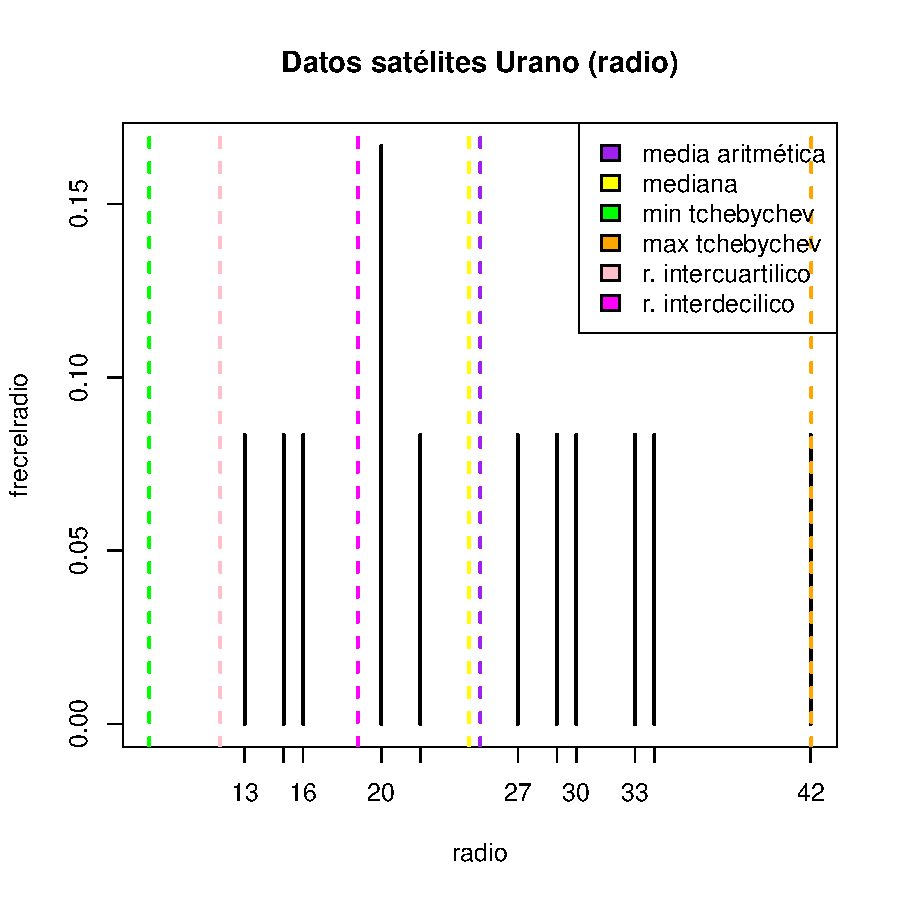
\includegraphics{Memoria-Figura 1}


\subsection{Otros cálculos}
Por último, vamos a realizar el cálculo de cálculos datos que pueden resultar relevantes a la hora 
de la analítica de datos, como pueden ser la obtención del rango del radio o su ordenación.

\subsubsection{Rango}
El rango de un conjunto de datos, consiste en la diferencia entre el valor más alto y el mínimo.
En R, lo hemos realizado de la siguiente forma:

\begin{Schunk}
\begin{Sinput}
> rangor<-max(radio)-min(radio)
> rangor
\end{Sinput}
\begin{Soutput}
[1] 29
\end{Soutput}
\end{Schunk}

\subsubsection{Ordenación}
Además, hemos añadido operaciones donde se muestran los datos de los radios ordenados ascendentemente y
descentemente:

\begin{Schunk}
\begin{Sinput}
> so<-s[order(radio),]
> so
\end{Sinput}
\begin{Soutput}
         Nombre Radio
1      Cordelia    13
12  Luna-1999U2    15
2        Ofelia    16
9  Luna-1986U10    20
11   Luna-999U1    20
3        Bianca    22
7     Rosalinda    27
5    Desdémona    29
10    Calíbano    30
4      Crésida    33
8       Belinda    34
6       Julieta    42
\end{Soutput}
\begin{Sinput}
> soi<-s[rev(order(radio)),]
> soi
\end{Sinput}
\begin{Soutput}
         Nombre Radio
6       Julieta    42
8       Belinda    34
4      Crésida    33
10    Calíbano    30
5    Desdémona    29
7     Rosalinda    27
3        Bianca    22
11   Luna-999U1    20
9  Luna-1986U10    20
2        Ofelia    16
12  Luna-1999U2    15
1      Cordelia    13
\end{Soutput}
\begin{Sinput}
> radio_ordenado<-radio[order(radio)]
> radio_ordenado
\end{Sinput}
\begin{Soutput}
 [1] 13 15 16 20 20 22 27 29 30 33 34 42
\end{Soutput}
\begin{Sinput}
> radio_ordenadorev<-radio[rev(order(radio))]
> radio_ordenadorev
\end{Sinput}
\begin{Soutput}
 [1] 42 34 33 30 29 27 22 20 20 16 15 13
\end{Soutput}
\end{Schunk}

\subsubsection{Lectura datos de Excel}
El último cálculo realizado ha sido leer datos de un archivo Excel. Para los análisis anteriores, leíamos los
datos de un archivo .txt y a través de la función read.table obteníamos los datos. A pesar del fácil manejo para 
la lectura de datos de un .txt, no es siempre la más adecuada, ya que cuando el número de columnas aumenta,
se hace más difícil la distribución de los datos en un .txt. Por este motivo, en un archivo Excel sería más 
útil esta distribución, por lo que hemos querido añadir la lectura de datos de un Excel.
Para ello, hemos transportado los  datos desde el txt hasta el Excel y 
ya en R, instalamos los siguientes paquetes y librería:


\begin{Schunk}
\begin{Sinput}
> install.packages("pastecs")
\end{Sinput}
\begin{Soutput}
package ‘pastecs’ successfully unpacked and MD5 sums checked

The downloaded binary packages are in
	C:\Users\Javier\AppData\Local\Temp\RtmpKes85j\downloaded_packages
\end{Soutput}
\begin{Sinput}
> install.packages("xlsx")
> library(xlsx)
\end{Sinput}
\end{Schunk}

Una vez incorporados, para la lectura realizamos lo siguiente:

\begin{Schunk}
\begin{Sinput}
> s_excel<-read.xlsx("satelites.xlsx",1)
\end{Sinput}
\end{Schunk}


\section{Análisis mpg de cardata}
Para este análisis, vamos a leer los datos del fichero cardata.sav y analizar la variable mpg. A diferencia del
análisis anterior, vamos a leer un fichar .sav (SPSS) y no .txt. Para la correcta lectura de este archivo, primero
tenemos que añadir la librería foreign. Tenemos dos opciones para añadirla. La primera, cosnsite en 
abrir el archivo RProfile y añadir "foreign" a la parte de dp, donde se encuentran
las librerías que se instalan por defecto al abrir R. La segunda opción sería ejecutar lo siguiente:

\begin{Schunk}
\begin{Sinput}
> library(foreign)
\end{Sinput}
\end{Schunk}

Una vez que tenemos la librería instalada, leemos el archivo cardata,sav y lo guardamos en una variable que
denominaremos cardata:

\begin{Schunk}
\begin{Sinput}
> cardata<-read.spss("cardata.sav")
\end{Sinput}
\end{Schunk}

Para facilitarnos los diferentes análisis, guardaremos los datos de mpg en una variable denominada mpg:

\begin{Schunk}
\begin{Sinput}
> mpg=cardata$mpg
> mpg
\end{Sinput}
\begin{Soutput}
  [1] 36.1 19.9 19.4 20.2 19.2 20.5 20.2 25.1 20.5 19.4 20.6 20.8 18.6 18.1 19.2
 [16] 17.7 18.1 17.5 30.0 30.9 23.2 23.8 21.5 19.8 22.3 20.2 20.6 17.0 17.6 16.5
 [31] 18.2 16.9 15.5 19.2 18.5 35.7 27.4 23.0 23.9 34.2 34.5 28.4 28.8 26.8 33.5
 [46] 32.1 28.0 26.4 24.3 19.1 27.9 23.6 27.2 26.6 25.8 23.5 30.0 39.0 34.7 34.4
 [61] 29.9 22.4 26.6 20.2 17.6 28.0 27.0 34.0 31.0 29.0 27.0 24.0 23.0 38.0 36.0
 [76] 25.0 38.0 26.0 22.0 36.0 27.0 27.0 32.0 28.0 31.0 43.1 20.3 17.0 21.6 16.2
 [91] 31.5 31.9 25.4 27.2 37.3 41.5 34.3 44.3 43.4 36.4 30.4 40.9 29.8 35.0 33.0
[106] 34.5 28.1   NA 30.7 36.0 44.0 32.8 39.4 36.1 27.5 27.2 21.1 23.9 29.5 34.1
[121] 31.8 38.1 37.2 29.8 31.3 37.0 32.2 46.6 40.8 44.6 33.8 32.7 23.7 32.4 39.1
[136] 35.1 32.3 37.0 37.7 34.1 33.7 32.4 32.9 31.6 25.4 24.2 37.0 31.0 36.0 36.0
[151] 34.0 38.0 32.0 38.0 32.0
\end{Soutput}
\end{Schunk}

Ahora, nos surge un problema que tenemos que resolver. En la columna mpg se encuentra algun valor nulo (NA), por
lo que si intentamos realizar algún cálculo con ella, el resultado sería NA, ya que no podría realizarse. 
Por lo tanto, debemos de deshacernos de estos valores nulos. Lo hacemos de la siguiente forma:

\begin{Schunk}
\begin{Sinput}
> mpg<-mpg[!is.na(mpg)]
> mpg
\end{Sinput}
\begin{Soutput}
  [1] 36.1 19.9 19.4 20.2 19.2 20.5 20.2 25.1 20.5 19.4 20.6 20.8 18.6 18.1 19.2
 [16] 17.7 18.1 17.5 30.0 30.9 23.2 23.8 21.5 19.8 22.3 20.2 20.6 17.0 17.6 16.5
 [31] 18.2 16.9 15.5 19.2 18.5 35.7 27.4 23.0 23.9 34.2 34.5 28.4 28.8 26.8 33.5
 [46] 32.1 28.0 26.4 24.3 19.1 27.9 23.6 27.2 26.6 25.8 23.5 30.0 39.0 34.7 34.4
 [61] 29.9 22.4 26.6 20.2 17.6 28.0 27.0 34.0 31.0 29.0 27.0 24.0 23.0 38.0 36.0
 [76] 25.0 38.0 26.0 22.0 36.0 27.0 27.0 32.0 28.0 31.0 43.1 20.3 17.0 21.6 16.2
 [91] 31.5 31.9 25.4 27.2 37.3 41.5 34.3 44.3 43.4 36.4 30.4 40.9 29.8 35.0 33.0
[106] 34.5 28.1 30.7 36.0 44.0 32.8 39.4 36.1 27.5 27.2 21.1 23.9 29.5 34.1 31.8
[121] 38.1 37.2 29.8 31.3 37.0 32.2 46.6 40.8 44.6 33.8 32.7 23.7 32.4 39.1 35.1
[136] 32.3 37.0 37.7 34.1 33.7 32.4 32.9 31.6 25.4 24.2 37.0 31.0 36.0 36.0 34.0
[151] 38.0 32.0 38.0 32.0
\end{Soutput}
\end{Schunk}

Una vez elminados estos valores nulos nos disponemos a hacer los análisis correspondientes (en este apartado no
realizaremos los análisis de frecuencias, ya que no es necesario).

\subsection{Segundo análisis datos: media aritmética y moda }

\subsubsection{Media aritmética}
Realizamos el cálculo de la media aritmética de mpg:

\begin{Schunk}
\begin{Sinput}
> m_mpg<-mean(mpg)
> m_mpg
\end{Sinput}
\begin{Soutput}
[1] 28.79351
\end{Soutput}
\end{Schunk}

\subsubsection{Moda}
Ahora, realizamos el cálculo de la moda. Para ello, antes tendremos que instalar el paquete y la librería
correspondientes:

\begin{Schunk}
\begin{Sinput}
> install.packages("modeest")
> library(modeest)
\end{Sinput}
\end{Schunk}


Ahora, ya podremos obtener la moda:

\begin{Schunk}
\begin{Sinput}
> modaMpg<-mfv(mpg)
> modaMpg
\end{Sinput}
\begin{Soutput}
[1] 36
\end{Soutput}
\end{Schunk}

\subsection{Tercer análisis de datos: medidas de dispersión}
Nos disponemos a realizar el cálculo de las medidas de dispersión de la variable mpg. Realizaremos el cálculo de
la desviación estándar y de la varianza.

\subsubsection{Desviación estándar}
Ahora, vamos a realizar el cálculo de la desviación estándar. Como hemos comentado en el análisis anterior,
la función que proporciona R no halla el resultado que más nos interesa, que sería la siguiente:

\begin{Schunk}
\begin{Sinput}
> sdR<-sd(mpg)
> sdR
\end{Sinput}
\begin{Soutput}
[1] 7.37721
\end{Soutput}
\end{Schunk}

Al no ser el resultado más interesante, vamos a utilizar la función creada en el análisis anterior (sd_nuestra). Para
ello, primero tenemos que abrir el archivo .R donde la función está creada:

\begin{Schunk}
\begin{Sinput}
> source("sd_nuestra.R")
\end{Sinput}
\end{Schunk}

Posteriormente, la usamos y hallamos el valor de la desviación estándar que nos interesa:

\begin{Schunk}
\begin{Sinput}
> sdN<-sd_nuestra(mpg)
> sdN
\end{Sinput}
\begin{Soutput}
[1] 7.353219
\end{Soutput}
\end{Schunk}

\subsubsection{Varianza}
Realizamos el cálculo de la varianza que nos proporciona R. Al igual que la desviación estándar,
no es la que más nos interesa:

\begin{Schunk}
\begin{Sinput}
> varR<-var(mpg)
> varR
\end{Sinput}
\begin{Soutput}
[1] 54.42323
\end{Soutput}
\end{Schunk}

Para calcular el resultado que nos interesa, obtenemos de forma teórica utilizamos 
la función, donde previamente abrimos el archivo de R donde fue creada:

\begin{Schunk}
\begin{Sinput}
> source("var_nuestra.R")
\end{Sinput}
\end{Schunk}

Una vez lo hemos abierto, podemos hallar la varianza con el procedimiento teórico:

\begin{Schunk}
\begin{Sinput}
> varN<-var_nuestra(mpg)
> varN
\end{Sinput}
\begin{Soutput}
[1] 54.06983
\end{Soutput}
\end{Schunk}

\subsection{Cuarto análisis de datos: medidas de ordenación}
Vamos a realizar las medidas de ordenación, es decir, la mediana y el cálculo de los cuantiles de la variable mpg.

\subsubsection{Mediana}
Realizamos el cálculo de la mediana de mpg:

\begin{Schunk}
\begin{Sinput}
> mdn_mpg<-median(mpg)
> mdn_mpg
\end{Sinput}
\begin{Soutput}
[1] 28.9
\end{Soutput}
\end{Schunk}

\subsubsection{Cuantiles}
Procedemos al cálculo de los cuartiles y deciles de mpg:

\begin{Schunk}
\begin{Sinput}
> q1<-quantile(mpg,0.25)
> q1 
\end{Sinput}
\begin{Soutput}
  25% 
22.55 
\end{Soutput}
\begin{Sinput}
> q2<-quantile(mpg,0.5)
> q2
\end{Sinput}
\begin{Soutput}
 50% 
28.9 
\end{Soutput}
\begin{Sinput}
> q3<-quantile(mpg,0.75)
> q3 
\end{Sinput}
\begin{Soutput}
   75% 
34.275 
\end{Soutput}
\begin{Sinput}
> dec1<-quantile(mpg,0.1)
> dec1
\end{Sinput}
\begin{Soutput}
  10% 
19.13 
\end{Soutput}
\begin{Sinput}
> dec2<-quantile(mpg,0.2)
> dec2
\end{Sinput}
\begin{Soutput}
 20% 
20.6 
\end{Soutput}
\begin{Sinput}
> dec3<-quantile(mpg,0.3)
> dec3
\end{Sinput}
\begin{Soutput}
  30% 
23.89 
\end{Soutput}
\begin{Sinput}
> dec4<-quantile(mpg,0.4)
> dec4
\end{Sinput}
\begin{Soutput}
40% 
 27 
\end{Soutput}
\begin{Sinput}
> dec5<-quantile(mpg,0.5)
> dec5
\end{Sinput}
\begin{Soutput}
 50% 
28.9 
\end{Soutput}
\begin{Sinput}
> dec6<-quantile(mpg,0.6)
> dec6
\end{Sinput}
\begin{Soutput}
  60% 
31.58 
\end{Soutput}
\begin{Sinput}
> dec7<-quantile(mpg,0.7)
> dec7
\end{Sinput}
\begin{Soutput}
  70% 
33.52 
\end{Soutput}
\begin{Sinput}
> dec8<-quantile(mpg,0.8)
> dec8
\end{Sinput}
\begin{Soutput}
  80% 
35.82 
\end{Soutput}
\begin{Sinput}
> dec9<-quantile(mpg,0.9)
> dec9 
\end{Sinput}
\begin{Soutput}
90% 
 38 
\end{Soutput}
\end{Schunk}

\subsubsection{Rango intercuartílico}
Calculamos el rango intercuantílico de mpg:

\begin{Schunk}
\begin{Sinput}
> rangintercuart<-q3-q1
> rangintercuart
\end{Sinput}
\begin{Soutput}
   75% 
11.725 
\end{Soutput}
\end{Schunk}
\subsubsection{Rango interdecil}
Calculamos el rango interdecil de mpg:

\begin{Schunk}
\begin{Sinput}
> ranginterdecil<-dec9-dec1
> ranginterdecil
\end{Sinput}
\begin{Soutput}
  90% 
18.87 
\end{Soutput}
\end{Schunk}

\subsection{Datos agrupados}
Ahora vamos a agrupar los datos de mpg por decenas al igual que con los satélites:

\begin{Schunk}
\begin{Sinput}
> mpg_agrupado<-cut(mpg, breaks=c(0,10,20,30,40,50))
> mpg_agrupado
\end{Sinput}
\begin{Soutput}
  [1] (30,40] (10,20] (10,20] (20,30] (10,20] (20,30] (20,30] (20,30] (20,30]
 [10] (10,20] (20,30] (20,30] (10,20] (10,20] (10,20] (10,20] (10,20] (10,20]
 [19] (20,30] (30,40] (20,30] (20,30] (20,30] (10,20] (20,30] (20,30] (20,30]
 [28] (10,20] (10,20] (10,20] (10,20] (10,20] (10,20] (10,20] (10,20] (30,40]
 [37] (20,30] (20,30] (20,30] (30,40] (30,40] (20,30] (20,30] (20,30] (30,40]
 [46] (30,40] (20,30] (20,30] (20,30] (10,20] (20,30] (20,30] (20,30] (20,30]
 [55] (20,30] (20,30] (20,30] (30,40] (30,40] (30,40] (20,30] (20,30] (20,30]
 [64] (20,30] (10,20] (20,30] (20,30] (30,40] (30,40] (20,30] (20,30] (20,30]
 [73] (20,30] (30,40] (30,40] (20,30] (30,40] (20,30] (20,30] (30,40] (20,30]
 [82] (20,30] (30,40] (20,30] (30,40] (40,50] (20,30] (10,20] (20,30] (10,20]
 [91] (30,40] (30,40] (20,30] (20,30] (30,40] (40,50] (30,40] (40,50] (40,50]
[100] (30,40] (30,40] (40,50] (20,30] (30,40] (30,40] (30,40] (20,30] (30,40]
[109] (30,40] (40,50] (30,40] (30,40] (30,40] (20,30] (20,30] (20,30] (20,30]
[118] (20,30] (30,40] (30,40] (30,40] (30,40] (20,30] (30,40] (30,40] (30,40]
[127] (40,50] (40,50] (40,50] (30,40] (30,40] (20,30] (30,40] (30,40] (30,40]
[136] (30,40] (30,40] (30,40] (30,40] (30,40] (30,40] (30,40] (30,40] (20,30]
[145] (20,30] (30,40] (30,40] (30,40] (30,40] (30,40] (30,40] (30,40] (30,40]
[154] (30,40]
Levels: (0,10] (10,20] (20,30] (30,40] (40,50]
\end{Soutput}
\end{Schunk}
A continuación, vamos a añadir etiquetas a cada valor agrupado:

\begin{Schunk}
\begin{Sinput}
> mpg_agrupado_etiqueta<-cut(mpg, breaks=c(0,10,20,30,40,50),
+  labels = c("Consumo muy bajo", 
+ "Consumo bajo", "Consumo medio", 
+ "Consumo alto", "Consumo muy alto"))
> mpg_agrupado_etiqueta
\end{Sinput}
\begin{Soutput}
  [1] Consumo alto     Consumo bajo     Consumo bajo     Consumo medio   
  [5] Consumo bajo     Consumo medio    Consumo medio    Consumo medio   
  [9] Consumo medio    Consumo bajo     Consumo medio    Consumo medio   
 [13] Consumo bajo     Consumo bajo     Consumo bajo     Consumo bajo    
 [17] Consumo bajo     Consumo bajo     Consumo medio    Consumo alto    
 [21] Consumo medio    Consumo medio    Consumo medio    Consumo bajo    
 [25] Consumo medio    Consumo medio    Consumo medio    Consumo bajo    
 [29] Consumo bajo     Consumo bajo     Consumo bajo     Consumo bajo    
 [33] Consumo bajo     Consumo bajo     Consumo bajo     Consumo alto    
 [37] Consumo medio    Consumo medio    Consumo medio    Consumo alto    
 [41] Consumo alto     Consumo medio    Consumo medio    Consumo medio   
 [45] Consumo alto     Consumo alto     Consumo medio    Consumo medio   
 [49] Consumo medio    Consumo bajo     Consumo medio    Consumo medio   
 [53] Consumo medio    Consumo medio    Consumo medio    Consumo medio   
 [57] Consumo medio    Consumo alto     Consumo alto     Consumo alto    
 [61] Consumo medio    Consumo medio    Consumo medio    Consumo medio   
 [65] Consumo bajo     Consumo medio    Consumo medio    Consumo alto    
 [69] Consumo alto     Consumo medio    Consumo medio    Consumo medio   
 [73] Consumo medio    Consumo alto     Consumo alto     Consumo medio   
 [77] Consumo alto     Consumo medio    Consumo medio    Consumo alto    
 [81] Consumo medio    Consumo medio    Consumo alto     Consumo medio   
 [85] Consumo alto     Consumo muy alto Consumo medio    Consumo bajo    
 [89] Consumo medio    Consumo bajo     Consumo alto     Consumo alto    
 [93] Consumo medio    Consumo medio    Consumo alto     Consumo muy alto
 [97] Consumo alto     Consumo muy alto Consumo muy alto Consumo alto    
[101] Consumo alto     Consumo muy alto Consumo medio    Consumo alto    
[105] Consumo alto     Consumo alto     Consumo medio    Consumo alto    
[109] Consumo alto     Consumo muy alto Consumo alto     Consumo alto    
[113] Consumo alto     Consumo medio    Consumo medio    Consumo medio   
[117] Consumo medio    Consumo medio    Consumo alto     Consumo alto    
[121] Consumo alto     Consumo alto     Consumo medio    Consumo alto    
[125] Consumo alto     Consumo alto     Consumo muy alto Consumo muy alto
[129] Consumo muy alto Consumo alto     Consumo alto     Consumo medio   
[133] Consumo alto     Consumo alto     Consumo alto     Consumo alto    
[137] Consumo alto     Consumo alto     Consumo alto     Consumo alto    
[141] Consumo alto     Consumo alto     Consumo alto     Consumo medio   
[145] Consumo medio    Consumo alto     Consumo alto     Consumo alto    
[149] Consumo alto     Consumo alto     Consumo alto     Consumo alto    
[153] Consumo alto     Consumo alto    
5 Levels: Consumo muy bajo Consumo bajo Consumo medio ... Consumo muy alto
\end{Soutput}
\end{Schunk}

\subsection{Visualización}
Vamos a representar gráficamente los cálculos estadísticos de mpg al igual que con los satélites:

\begin{Schunk}
\begin{Sinput}
> mintchebychev <- m_mpg-2*sdN
> mintchebychev
\end{Sinput}
\begin{Soutput}
[1] 14.08707
\end{Soutput}
\begin{Sinput}
> maxtchebychev <- m_mpg+2*sdN
> maxtchebychev
\end{Sinput}
\begin{Soutput}
[1] 43.49994
\end{Soutput}
\end{Schunk}
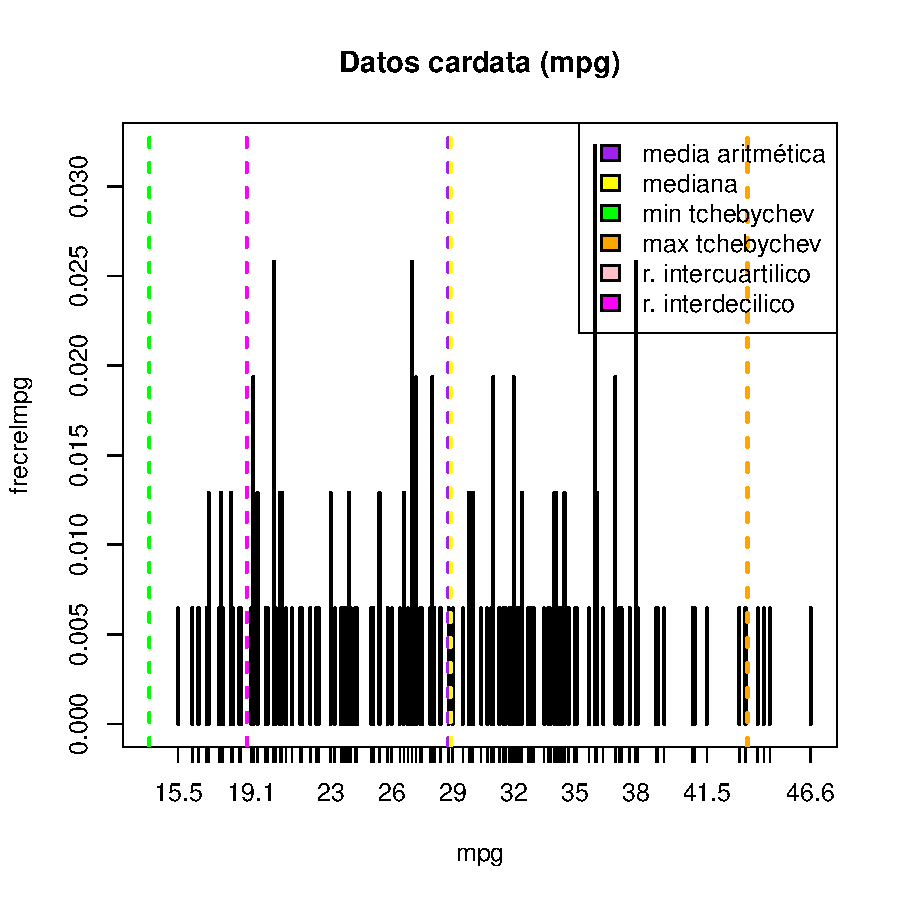
\includegraphics{Memoria-Figura 2}

\subsection{Otros cálculos}

\subsubsection{Rango}
Realizamos el rango de los datos de mpg:

\begin{Schunk}
\begin{Sinput}
> rangompg<-max(mpg)-min(mpg)
> rangompg
\end{Sinput}
\begin{Soutput}
[1] 31.1
\end{Soutput}
\end{Schunk}


\subsubsection{Ordenación}
Ordenamos mpg en orden ascendente:

\begin{Schunk}
\begin{Sinput}
> mpg_ordenado<-mpg[order(mpg)]
> mpg_ordenado
\end{Sinput}
\begin{Soutput}
  [1] 15.5 16.2 16.5 16.9 17.0 17.0 17.5 17.6 17.6 17.7 18.1 18.1 18.2 18.5 18.6
 [16] 19.1 19.2 19.2 19.2 19.4 19.4 19.8 19.9 20.2 20.2 20.2 20.2 20.3 20.5 20.5
 [31] 20.6 20.6 20.8 21.1 21.5 21.6 22.0 22.3 22.4 23.0 23.0 23.2 23.5 23.6 23.7
 [46] 23.8 23.9 23.9 24.0 24.2 24.3 25.0 25.1 25.4 25.4 25.8 26.0 26.4 26.6 26.6
 [61] 26.8 27.0 27.0 27.0 27.0 27.2 27.2 27.2 27.4 27.5 27.9 28.0 28.0 28.0 28.1
 [76] 28.4 28.8 29.0 29.5 29.8 29.8 29.9 30.0 30.0 30.4 30.7 30.9 31.0 31.0 31.0
 [91] 31.3 31.5 31.6 31.8 31.9 32.0 32.0 32.0 32.1 32.2 32.3 32.4 32.4 32.7 32.8
[106] 32.9 33.0 33.5 33.7 33.8 34.0 34.0 34.1 34.1 34.2 34.3 34.4 34.5 34.5 34.7
[121] 35.0 35.1 35.7 36.0 36.0 36.0 36.0 36.0 36.1 36.1 36.4 37.0 37.0 37.0 37.2
[136] 37.3 37.7 38.0 38.0 38.0 38.0 38.1 39.0 39.1 39.4 40.8 40.9 41.5 43.1 43.4
[151] 44.0 44.3 44.6 46.6
\end{Soutput}
\end{Schunk}


\subsubsection{Lectura datos de Excel}
Igual que el análisis anterior, en este script volvemos a realizar la lectura de un archivo Excel.
En este análisis, se puede comprobar mejor la utilidad que tiene leer archivos de Excel, ya que
el número de columnas es elevado y en un archivo Excel se organiza mejor. Para ello, hemos transformado
el archivo.sav en Excel y hemos realizado lo mismo que anteriormente. Instalamos los siguientes paquetes
y librerías:


\begin{Schunk}
\begin{Sinput}
> install.packages("pastecs")
\end{Sinput}
\begin{Soutput}
package ‘pastecs’ successfully unpacked and MD5 sums checked

The downloaded binary packages are in
	C:\Users\Javier\AppData\Local\Temp\RtmpKes85j\downloaded_packages
\end{Soutput}
\begin{Sinput}
> install.packages("xlsx")
> library(xlsx)
\end{Sinput}
\end{Schunk}

Y una vez incorporados, realizamos lo siguiente para la lectura:

\begin{Schunk}
\begin{Sinput}
> cardata_excel<-read.xlsx("cardata.xlsx",1)
\end{Sinput}
\end{Schunk}


\section{Conclusión}
En esta práctica se ha aprendido a como realizar los cálculos básicos de estadística
pedidos en el enunciado, como pueden ser la media aritmética o medidas de dispersión y 
ordenación, utilizando el lenguaje R y su IDE Rgui. Además, hemos añadido 
modificaciones sobre lo pedido. Por ejemplo, hemos añadido el cálculo de la moda,
hemos agrupado los datos y calculado sus frecuencias y además rangos intercuatilico
e interdecil. También, se han realizado lectura de datos de otros ficheros 
diferentes a los proporcionados por el enunciado (txt y sav) como por ejemplo 
un archivo excel (xlsx). Por último, para la realización de esta memoria, 
hemos utilizado las herramientas Sweave y Latex para la producción de documentos 
científicos relacionados con los estudios de datos.
\end{document}
